% !TEX TS-program = pdflatex
% !TEX encoding = UTF-8
\documentclass[conference]{IEEEtran}
\usepackage[utf8]{inputenc}
\usepackage[T1]{fontenc}
\usepackage[vietnamese]{babel}
\usepackage{graphicx}
\usepackage{hyperref}
\usepackage{cite}
\usepackage{amsmath,amssymb}
\usepackage{booktabs}
\usepackage{caption}
\usepackage{subcaption}
\usepackage{url}
\usepackage{multirow}
\usepackage{array}
\usepackage{tabularx}
\captionsetup[figure]{labelfont=bf,labelsep=colon}
\captionsetup[table]{labelfont=bf,labelsep=colon}

\author{
    \IEEEauthorblockN{Đỗ Đình Vinh, Phạm Thùy Dương, Hà Phạm Mai Linh và Ngô Mạnh Cường\IEEEauthorrefmark{1}}
    \IEEEauthorblockA{Khoa Công nghệ Thông tin, Trường Đại học Thăng Long, Hà Nội, Việt Nam\\[3pt]
    Email: \{haivinh2092006, pduonng29, hpmlinh26\}@gmail.com\\[3pt]
    \IEEEauthorrefmark{1}Giảng viên hướng dẫn. Tác giả liên hệ: cuongnm@thanglong.edu.vn}a
}

\begin{document}

\title{Nghiên cứu và triển khai mô hình phân vùng ảnh sử dụng học sâu trên Raspberry Pi}
\maketitle

% ========== TÓM TẮT ==========
\begin{abstract}
Phân vùng ảnh ngữ nghĩa sử dụng học sâu đã đạt được độ chính xác vượt trội trên các nền tảng GPU hiệu năng cao; tuy nhiên, việc triển khai các mô hình này trên thiết bị biên với tài nguyên hạn chế vẫn là một thách thức lớn. Phần lớn các nghiên cứu hiện tại chỉ đánh giá các chỉ số phân vùng (ví dụ: mIoU) trên máy chủ trang bị GPU, trong khi bỏ qua các chỉ số triển khai thực tế như tốc độ suy luận (FPS), độ trễ và mức tiêu thụ bộ nhớ trên phần cứng đích. Bài báo này giải quyết khoảng trống đó bằng cách trình bày một quy trình triển khai end-to-end hoàn chỉnh cho mô hình phân vùng ngữ nghĩa nhẹ trên Raspberry Pi~4, hướng đến ứng dụng phân vùng bệnh thực vật trong nông nghiệp chính xác. Chúng tôi sử dụng kiến trúc Fast-SCNN làm mô hình xương sống, huấn luyện trên tập dữ liệu PlantSeg~v7 và áp dụng lượng tử hóa INT8 sau huấn luyện thông qua TensorFlow Lite, giảm 75\% dung lượng mô hình (từ 2,5~MB xuống 636~KB). Kết quả đánh giá trực tiếp trên CPU ARM Cortex-A72 cho thấy mô hình sau lượng tử hóa đạt tốc độ suy luận 24,79~FPS với độ trễ trung bình 40,33~ms, đáp ứng yêu cầu xử lý gần thời gian thực, đồng thời duy trì chỉ số IoU ở mức 0,667. Khác với các công trình trước đây chỉ kiểm chứng trên GPU máy bàn, toàn bộ quá trình đánh giá của chúng tôi được thực hiện trên thiết bị đích, báo cáo các chỉ số FPS, mức sử dụng RAM và độ trễ từng khung hình trong điều kiện thực tế. Kết quả khẳng định tính khả thi của việc triển khai phân vùng ảnh chính xác, độ trễ thấp trên phần cứng có giá dưới 50~USD mà không cần kết nối đám mây, mở đường cho các giải pháp Edge~AI có khả năng mở rộng trong giám sát nông nghiệp.
\end{abstract}

\begin{IEEEkeywords}
Phân vùng ảnh ngữ nghĩa, Edge AI, Raspberry Pi, Fast-SCNN, lượng tử hóa INT8, phát hiện bệnh thực vật, nông nghiệp thông minh
\end{IEEEkeywords}

% ========== 1. GIỚI THIỆU ==========
\section{Giới thiệu}

\subsection{Bối cảnh và Động lực nghiên cứu}

Phân vùng ảnh ngữ nghĩa (Semantic Segmentation) --- nhiệm vụ gán nhãn lớp cho từng điểm ảnh trong một bức ảnh --- là một trong những bài toán nền tảng của thị giác máy tính hiện đại, với phạm vi ứng dụng rộng rãi trong lái xe tự hành, hình ảnh y khoa và nông nghiệp thông minh~\cite{ngugi2020image,chen2018encoder}. Các kiến trúc tiên tiến như DeepLabV3+~\cite{chen2018encoder} và HRNet~\cite{wang2020high} thường xuyên đạt điểm mIoU (mean Intersection-over-Union) vượt 80\% trên các tập dữ liệu chuẩn. Tuy nhiên, các mô hình này thường chứa hàng chục triệu tham số và đòi hỏi GPU mạnh để suy luận theo thời gian thực, khiến chúng không phù hợp để triển khai trên các thiết bị biên --- nơi tài nguyên tính toán, bộ nhớ và năng lượng đều bị giới hạn nghiêm ngặt.

Trong lĩnh vực nông nghiệp, việc phát hiện sớm và chính xác bệnh trên cây trồng đóng vai trò then chốt trong việc giảm thiểu tổn thất mùa vụ và hạn chế sử dụng thuốc trừ sâu~\cite{mohanty2016using}. Các hệ thống thị giác biên được lắp đặt trực tiếp tại đồng ruộng có thể cung cấp chẩn đoán kịp thời, tại chỗ mà không phụ thuộc vào hạ tầng đám mây --- một yêu cầu thiết yếu tại các vùng nông thôn nơi băng thông mạng bị hạn chế hoặc không khả dụng. Raspberry Pi~4, được trang bị CPU ARM Cortex-A72 bốn nhân xung nhịp 1,5~GHz và tối đa 8~GB RAM LPDDR4, là một nền tảng hấp dẫn nhờ chi phí thấp (dưới 50~USD), kích thước nhỏ gọn và hệ sinh thái phần mềm phong phú. Tuy nhiên, thiết bị này không tích hợp GPU hay Bộ xử lý thần kinh chuyên dụng (NPU), đặt ra thách thức cơ bản cho việc chạy các mô hình học sâu ở tốc độ khung hình tương tác.

\subsection{Khoảng trống nghiên cứu}

Tổng quan tài liệu cho thấy tồn tại một khoảng cách dai dẳng giữa hiệu quả mô hình trên lý thuyết và hiệu năng triển khai thực tế. Đa số các nghiên cứu về phân vùng nhẹ~\cite{zhao2021lightweight,bisenet2018} đánh giá mô hình trên GPU máy bàn hoặc máy chủ (ví dụ: NVIDIA GTX 1080 Ti, Tesla V100) và chỉ báo cáo mIoU cùng với số lượng phép toán lý thuyết (FLOPs) hoặc số lượng tham số. Mặc dù các chỉ số này hữu ích cho việc so sánh kiến trúc mô hình một cách đơn lẻ, chúng không phản ánh được hành vi thực tế trên phần cứng biên --- nơi các yếu tố như băng thông bộ nhớ, cấu trúc bộ nhớ đệm, mức độ hỗ trợ toán tử trong các engine suy luận và hiện tượng giảm xung nhịp do nhiệt ảnh hưởng đáng kể đến thông lượng xử lý. Do đó, các nhà nghiên cứu và kỹ sư muốn triển khai những mô hình này trên thiết bị như Raspberry Pi không có các mốc hiệu năng đáng tin cậy để tham khảo.

Hơn nữa, những nghiên cứu có đánh giá trên nền tảng nhúng thường chỉ giới hạn ở bài toán phân loại ảnh hoặc phát hiện đối tượng~\cite{han2015learning, hinton2015distilling}, trong khi rất ít công trình đề cập đến phân vùng ở mức điểm ảnh --- một bài toán đòi hỏi tính toán cao hơn nhiều do yêu cầu dự đoán dày đặc trên toàn bộ ảnh.

\subsection{Mục tiêu và Đóng góp}

Bài báo này nhằm thu hẹp khoảng cách giữa đánh giá trên GPU và triển khai thực tế trên thiết bị biên, thông qua việc trình bày một quy trình phân vùng ngữ nghĩa hoàn chỉnh, có thể tái tạo trên Raspberry Pi~4. Cụ thể, các đóng góp chính của chúng tôi bao gồm:
\begin{enumerate}
  \item \textbf{Quy trình triển khai end-to-end.} Chúng tôi thiết kế và triển khai một luồng xử lý đầy đủ bao gồm chuẩn bị dữ liệu, huấn luyện mô hình, lượng tử hóa INT8 sau huấn luyện và suy luận trên thiết bị sử dụng TensorFlow Lite, trên tập dữ liệu bệnh thực vật PlantSeg~v7.
  \item \textbf{Đánh giá toàn diện trên thiết bị đích.} Khác với các công trình trước đây, chúng tôi đánh giá mô hình đã triển khai trực tiếp trên CPU ARM Cortex-A72 của Raspberry Pi~4, báo cáo các chỉ số thực tế bao gồm thông lượng suy luận (FPS), độ trễ từng khung hình (ms), mức tiêu thụ RAM đỉnh và độ chính xác phân vùng (IoU) --- cung cấp cái nhìn toàn diện về tính khả thi triển khai.
  \item \textbf{Phân tích tác động của lượng tử hóa.} Chúng tôi đánh giá định lượng các đánh đổi do lượng tử hóa INT8 mang lại, chứng minh mức giảm 75\% dung lượng mô hình (từ 2,5~MB xuống 636~KB) với mức suy giảm độ chính xác chấp nhận được, cho phép mô hình hoạt động trong giới hạn bộ nhớ khắt khe của thiết bị biên.
  \item \textbf{Chứng minh tính khả thi thực tiễn.} Chúng tôi cho thấy việc phân vùng gần thời gian thực (24,79~FPS, độ trễ 40,33~ms) hoàn toàn khả thi trên phần cứng thương mại có giá dưới 50~USD, không phụ thuộc vào kết nối đám mây hay bộ tăng tốc chuyên dụng.
\end{enumerate}

\subsection{Cấu trúc bài báo}

Phần còn lại của bài báo được tổ chức như sau. Mục~2 tổng quan các công trình liên quan về kiến trúc phân vùng nhẹ và chiến lược triển khai biên. Mục~3 mô tả phương pháp đề xuất, bao gồm tập dữ liệu, kiến trúc mô hình, quy trình lượng tử hóa và thiết lập triển khai. Mục~4 trình bày kết quả thực nghiệm và phân tích. Mục~5 kết luận và đề xuất hướng phát triển tương lai.


% ========== 2. CƠ SỞ LÝ THUYẾT VÀ NGHIÊN CỨU LIÊN QUAN ==========
\section{Cơ sở lý thuyết và Nghiên cứu liên quan}

\subsection{Phân vùng ảnh ngữ nghĩa và các mô hình nhẹ}

\subsubsection{Sự ra đời của Mạng Tích chập Toàn phần (FCN)}

Phân vùng ảnh ngữ nghĩa (Semantic Segmentation) là bài toán gán nhãn lớp cho từng điểm ảnh trong một bức ảnh đầu vào. Bước đột phá mang tính nền tảng trong lĩnh vực này là công trình Fully Convolutional Network (FCN) do Long và cộng sự đề xuất vào năm 2015~\cite{long2015fully}. FCN là kiến trúc đầu tiên loại bỏ hoàn toàn các tầng kết nối đầy đủ (Fully Connected Layers) trong mạng phân loại truyền thống, thay thế bằng các tầng tích chập, cho phép mạng chấp nhận ảnh đầu vào có kích thước tùy ý và tạo ra bản đồ phân vùng dày đặc (dense prediction map). Ý tưởng cốt lõi của FCN --- kiến trúc mã hóa-giải mã (Encoder-Decoder) kết hợp với kết nối tắt (skip connections) để phục hồi thông tin không gian --- đã trở thành khuôn mẫu cho hầu hết các kiến trúc phân vùng sau này, bao gồm U-Net~\cite{ronneberger2015u}, SegNet~\cite{badrinarayanan2017segnet}, DeepLabV3+~\cite{chen2018encoder} và PSPNet~\cite{zhao2017pyramid}.

Tuy nhiên, các kiến trúc kế thừa FCN ngày càng phức tạp với hàng chục đến hàng trăm triệu tham số, đòi hỏi GPU hiệu năng cao để đạt tốc độ suy luận theo thời gian thực. Điều này đã thúc đẩy một hướng nghiên cứu song song tập trung vào việc thiết kế các mô hình phân vùng nhẹ (lightweight segmentation models), phù hợp cho triển khai trên các thiết bị biên có tài nguyên hạn chế.

\subsubsection{Các mô hình phân vùng nhẹ cho thiết bị biên}

Một số kiến trúc nhẹ tiêu biểu đã được đề xuất nhằm giải quyết bài toán phân vùng thời gian thực trên phần cứng hạn chế:

\textbf{ENet (Efficient Neural Network)}~\cite{enet2016} là một trong những kiến trúc tiên phong theo hướng phân vùng nhẹ, được thiết kế với mục tiêu tối ưu hóa tốc độ suy luận. ENet sử dụng kiến trúc bất đối xứng với bộ mã hóa lớn hơn đáng kể so với bộ giải mã, kết hợp các kỹ thuật như tích chập giãn (dilated convolutions) và phân tách tầng sớm (early downsampling) để giảm chi phí tính toán. Với khoảng 0,36~M tham số, ENet đạt tốc độ suy luận cao nhưng phải đánh đổi đáng kể về độ chính xác --- chỉ số mIoU trên Cityscapes chỉ đạt khoảng 58,3\%, thấp hơn nhiều so với các mô hình cùng phân khúc.

\textbf{BiSeNet (Bilateral Segmentation Network)}~\cite{bisenet2018} đề xuất một kiến trúc hai nhánh: nhánh không gian (Spatial Path) giữ lại thông tin chi tiết ở độ phân giải cao, trong khi nhánh ngữ cảnh (Context Path) sử dụng mạng backbone nhẹ để trích xuất trường tiếp nhận rộng. Hai nhánh được kết hợp thông qua cơ chế Feature Fusion Module. BiSeNet đạt mIoU cạnh tranh (68,4\% trên Cityscapes) với tốc độ 105,8~FPS trên GPU. Tuy nhiên, kiến trúc hai nhánh làm tăng mức sử dụng bộ nhớ và độ phức tạp triển khai trên các thiết bị biên không có GPU.

\textbf{Fast-SCNN (Fast Segmentation Convolutional Neural Network)}~\cite{fastscnn2019} được thiết kế đặc biệt cho suy luận thời gian thực trên thiết bị có tài nguyên hạn chế. Kiến trúc này kết hợp một mô-đun trích xuất đặc trưng dùng chung (Learning to Downsample) với mô-đun bộ trích xuất đặc trưng toàn cục (Global Feature Extractor) dựa trên các khối nghịch đảo thặng dư (Inverted Residual Bottleneck) kế thừa từ MobileNetV2~\cite{mobilenetv22018}, và một mô-đun kết hợp đặc trưng (Feature Fusion Module). Với chỉ 1,11~M tham số, Fast-SCNN đạt 68,0\% mIoU trên Cityscapes và tốc độ suy luận tham chiếu 123,5~FPS trên GPU --- thể hiện sự cân bằng tối ưu giữa độ chính xác, tốc độ và dung lượng mô hình.

Bảng~\ref{tab:compare_models} tóm tắt so sánh các kiến trúc nhẹ nêu trên.

\begin{table}[htbp]
\centering
\caption{So sánh các mô hình phân vùng nhẹ trên tập Cityscapes}
\label{tab:compare_models}
\begin{tabular}{lcccc}
\toprule
\textbf{Mô hình} & \textbf{Tham số} & \textbf{mIoU} & \textbf{FPS} & \textbf{Đặc điểm} \\
\midrule
ENet      & 0,36M  & 58,3\% & 135,4 & Siêu nhẹ, chính xác hạn chế \\
BiSeNet   & 5,80M  & 68,4\% & 105,8 & Hai nhánh, tốn bộ nhớ \\
Fast-SCNN & 1,11M  & 68,0\% & 123,5 & Một nhánh, cân bằng tốt \\
\bottomrule
\end{tabular}
\end{table}

\subsubsection{Lý do lựa chọn Fast-SCNN}

Trong nghiên cứu này, chúng tôi lựa chọn Fast-SCNN làm kiến trúc chính cho triển khai trên Raspberry Pi~4, dựa trên các lý do sau:

\begin{enumerate}
  \item \textbf{Số lượng tham số tối ưu.} Với chỉ 1,11~M tham số, Fast-SCNN nhỏ hơn BiSeNet gấp 5 lần (5,80M) trong khi đạt mIoU tương đương (68,0\% so với 68,4\%). So với ENet (0,36M), Fast-SCNN có số tham số lớn hơn nhưng vượt trội rõ rệt về độ chính xác (chênh lệch gần 10\% mIoU).
  \item \textbf{Kiến trúc một nhánh.} Khác với BiSeNet sử dụng hai nhánh xử lý song song đòi hỏi cấp phát bộ nhớ kép, Fast-SCNN áp dụng kiến trúc một nhánh duy nhất. Điều này giúp giảm đáng kể mức tiêu thụ RAM --- yếu tố cực kỳ quan trọng trên Raspberry Pi~4 với bộ nhớ hạn chế và không có GPU để xử lý song song hiệu quả.
  \item \textbf{Tốc độ suy luận cạnh tranh.} Fast-SCNN đạt 123,5~FPS trên GPU tham chiếu, cao hơn BiSeNet (105,8~FPS) và chỉ thấp hơn nhẹ so với ENet (135,4~FPS). Tốc độ tham chiếu cao trên GPU cho thấy mô hình có số lượng phép toán thấp, tạo tiền đề thuận lợi cho suy luận hiệu quả khi chuyển đổi sang CPU ARM.
  \item \textbf{Khả năng tương thích với lượng tử hóa.} Kiến trúc Fast-SCNN chủ yếu sử dụng các toán tử chuẩn (tích chập tách biệt theo chiều sâu, tích chập điểm, cộng gộp trung bình) được TensorFlow Lite hỗ trợ đầy đủ, đảm bảo quá trình lượng tử hóa INT8 diễn ra thuận lợi mà không cần thay đổi kiến trúc.
\end{enumerate}

\subsection{Các kỹ thuật tối ưu hóa mô hình cho thiết bị biên}

Để triển khai mô hình học sâu trên thiết bị biên có tài nguyên hạn chế, ba kỹ thuật tối ưu hóa chính thường được sử dụng: lượng tử hóa (Quantization), cắt tỉa (Pruning) và chưng cất tri thức (Knowledge Distillation).

\subsubsection{Cắt tỉa mô hình (Pruning)}

Cắt tỉa mô hình~\cite{han2015learning} là kỹ thuật loại bỏ các trọng số hoặc toàn bộ bộ lọc tích chập có đóng góp thấp đến kết quả đầu ra. Phương pháp này có thể phân thành hai loại: cắt tỉa phi cấu trúc (loại bỏ trọng số đơn lẻ, tạo ma trận thưa) và cắt tỉa có cấu trúc (loại bỏ toàn bộ kênh hoặc bộ lọc). Mặc dù cắt tỉa có thể giảm đáng kể số lượng tham số, phương pháp này thường yêu cầu tái huấn luyện (fine-tuning) sau khi cắt tỉa và việc tận dụng lợi ích tốc độ từ ma trận thưa trên CPU ARM vẫn còn hạn chế do thiếu hỗ trợ phần cứng chuyên biệt.

\subsubsection{Chưng cất tri thức (Knowledge Distillation)}

Chưng cất tri thức~\cite{hinton2015distilling} là kỹ thuật huấn luyện một mô hình nhỏ (student) để bắt chước hành vi của một mô hình lớn hơn, chính xác hơn (teacher). Mô hình student học không chỉ từ nhãn cứng (hard labels) mà còn từ phân phối xác suất đầu ra mềm (soft labels) của mô hình teacher, giúp thu được kiến thức ẩn (dark knowledge). Phương pháp này hiệu quả trong việc nâng cao độ chính xác của mô hình nhỏ, nhưng đòi hỏi sự tồn tại của một mô hình teacher đã được huấn luyện tốt và quy trình huấn luyện phức tạp hơn.

\subsubsection{Lượng tử hóa sau huấn luyện (Post-Training Quantization)}

Lượng tử hóa~\cite{jacob2018quantization} là kỹ thuật giảm độ chính xác số học của các trọng số và phép tính kích hoạt trong mô hình từ dạng dấu phẩy động 32-bit (FP32) sang biểu diễn có độ chính xác thấp hơn, phổ biến nhất là số nguyên 8-bit (INT8). Quá trình ánh xạ từ FP32 sang INT8 được thực hiện thông qua phép biến đổi affine tuyến tính:
\begin{equation}
q = \text{round}\left(\frac{r}{s}\right) + z
\end{equation}
trong đó $r$ là giá trị thực FP32 cần lượng tử hóa, $s$ (scale) là hệ số tỷ lệ được tính dựa trên phạm vi giá trị thực ($r_{min}$, $r_{max}$), $z$ (zero-point) là điểm không đảm bảo giá trị thực 0 được ánh xạ chính xác sang miền INT8, và $q$ là giá trị INT8 kết quả nằm trong khoảng $[-128, 127]$ hoặc $[0, 255]$.

Hệ số tỷ lệ $s$ được xác định bởi:
\begin{equation}
s = \frac{r_{\max} - r_{\min}}{q_{\max} - q_{\min}}
\end{equation}

Lượng tử hóa sau huấn luyện (Post-Training Quantization --- PTQ) thực hiện quá trình chuyển đổi này mà \textbf{không cần tái huấn luyện mô hình}. Thay vào đó, PTQ sử dụng một tập dữ liệu hiệu chuẩn đại diện nhỏ để xác định phạm vi giá trị cho từng tầng mạng, từ đó tính toán các tham số $s$ và $z$ tối ưu. Ưu điểm chính của PTQ bao gồm: giảm khoảng 75\% dung lượng lưu trữ; tăng tốc suy luận nhờ tập lệnh NEON SIMD trên ARM Cortex-A72; giảm tiêu thụ bộ nhớ và năng lượng.

\subsubsection{Lý do lựa chọn INT8 PTQ}

Chúng tôi lựa chọn PTQ INT8 làm phương pháp tối ưu hóa chính dựa trên các cân nhắc sau:
\begin{enumerate}
  \item \textbf{Hiệu quả giảm dung lượng trực tiếp.} PTQ INT8 giảm dung lượng mô hình Fast-SCNN từ 2,5~MB xuống 636~KB (giảm 75\%), đáp ứng giới hạn bộ nhớ trên Raspberry Pi mà không cần thay đổi kiến trúc mạng.
  \item \textbf{Không yêu cầu tái huấn luyện.} So với Quantization-Aware Training (QAT), cắt tỉa kết hợp fine-tuning, hay chưng cất tri thức --- tất cả đều đòi hỏi quá trình tái huấn luyện tốn thời gian và tài nguyên GPU --- PTQ cho phép chuyển đổi mô hình đã huấn luyện chỉ với một tập hiệu chuẩn nhỏ.
  \item \textbf{Tương thích phần cứng tốt.} CPU ARM Cortex-A72 trên Raspberry Pi~4 hỗ trợ tập lệnh NEON SIMD, cho phép thực hiện các phép toán INT8 song song hiệu quả. TensorFlow Lite runtime khai thác trực tiếp khả năng này để tăng tốc suy luận.
  \item \textbf{Cân bằng tốc độ tối ưu hóa và chất lượng.} Kết quả thực nghiệm cho thấy mô hình sau lượng tử hóa vẫn duy trì IoU ở mức 0,667, chứng tỏ mức suy giảm chất lượng nằm trong ngưỡng chấp nhận được cho ứng dụng phân vùng bệnh thực vật tại hiện trường.
\end{enumerate}

\subsection{Tổng kết chương}

Qua phân tích tổng quan, có thể thấy rằng mặc dù nhiều kiến trúc phân vùng nhẹ và kỹ thuật tối ưu hóa đã được đề xuất, vẫn thiếu vắng các nghiên cứu đánh giá end-to-end trên thiết bị biên thực tế, đặc biệt trên nền tảng CPU thuần như Raspberry Pi~4. Sự kết hợp giữa Fast-SCNN --- kiến trúc đạt cân bằng tối ưu giữa tốc độ, độ chính xác và dung lượng --- với lượng tử hóa INT8 PTQ --- phương pháp tối ưu hóa đơn giản, hiệu quả và tương thích phần cứng --- tạo nền tảng kỹ thuật vững chắc cho quy trình triển khai được trình bày trong các mục tiếp theo.


% ========== 3. PHƯƠNG PHÁP ĐỀ XUẤT ==========
\section{Phương pháp đề xuất}

Mục này trình bày chi tiết quy trình kỹ thuật end-to-end của nghiên cứu, bao gồm bốn giai đoạn chính: (1)~chuẩn bị và tiền xử lý dữ liệu, (2)~thiết kế và huấn luyện mô hình, (3)~lượng tử hóa mô hình, và (4)~triển khai suy luận trên thiết bị đích.

\subsection{Bộ dữ liệu và Tiền xử lý}

\subsubsection{Bộ dữ liệu PlantSeg v7}

Nghiên cứu sử dụng bộ dữ liệu PlantSeg~v7, một tập dữ liệu phân vùng bệnh thực vật quy mô lớn với tổng dung lượng 1,1~GB, bao gồm 7.774 ảnh chụp lá cây mắc các loại bệnh khác nhau cùng các mặt nạ phân vùng (segmentation masks) tương ứng. Mỗi cặp ảnh-mặt nạ cho phép mô hình học cách phân biệt vùng lá bị nhiễm bệnh với vùng lá khỏe mạnh và nền ảnh ở mức điểm ảnh.

\subsubsection{Phân chia tập dữ liệu}

Bộ dữ liệu được phân chia thành ba tập con theo tỉ lệ được trình bày trong Bảng~\ref{tab:dataset_split}. Việc phân chia đảm bảo nguyên tắc: tập kiểm tra hoàn toàn độc lập với quá trình huấn luyện và lựa chọn mô hình, nhằm phản ánh khả năng tổng quát hóa thực tế.

\begin{table}[htbp]
\centering
\caption{Phân chia tập dữ liệu PlantSeg v7}
\label{tab:dataset_split}
\begin{tabular}{lccp{3.2cm}}
\toprule
\textbf{Tập} & \textbf{Số ảnh} & \textbf{Tỉ lệ} & \textbf{Mục đích} \\
\midrule
Huấn luyện   & 5.367 & 69\% & Học các tham số mô hình \\
Xác thực     & 855   & 11\% & Theo dõi hiệu suất, điều chỉnh siêu tham số, dừng sớm \\
Kiểm tra     & 1.552 & 20\% & Đánh giá hiệu suất cuối cùng \\
\bottomrule
\end{tabular}
\end{table}

\subsubsection{Tiền xử lý dữ liệu}

Tất cả ảnh đầu vào và mặt nạ phân vùng tương ứng được tiền xử lý thống nhất qua hai bước:

\begin{enumerate}
  \item \textbf{Thay đổi kích thước (Resize).} Mọi ảnh được chuyển về kích thước cố định $256 \times 256$ điểm ảnh sử dụng phép nội suy song tuyến tính (bilinear interpolation) cho ảnh gốc và phép nội suy lân cận gần nhất (nearest-neighbor interpolation) cho mặt nạ, nhằm bảo toàn các giá trị nhãn rời rạc. Kích thước $256 \times 256$ được lựa chọn dựa trên sự cân bằng giữa độ phân giải đủ để nhận diện đặc trưng bệnh và yêu cầu giảm chi phí tính toán trên thiết bị biên.
  \item \textbf{Chuẩn hóa giá trị điểm ảnh.} Giá trị cường độ điểm ảnh của ảnh đầu vào được chuẩn hóa từ khoảng $[0, 255]$ về khoảng $[0, 1]$ bằng phép chia cho 255. Việc chuẩn hóa giúp ổn định quá trình huấn luyện, tăng tốc hội tụ gradient và đảm bảo tương thích với hàm kích hoạt trong mạng.
\end{enumerate}

\subsection{Kiến trúc mô hình Fast-SCNN}

\subsubsection{Tổng quan kiến trúc}

Fast-SCNN~\cite{fastscnn2019} là một kiến trúc phân vùng ngữ nghĩa nhẹ được thiết kế cho suy luận thời gian thực trên thiết bị hạn chế tài nguyên. Kiến trúc bao gồm bốn mô-đun chính:

\textbf{Mô-đun Learning to Downsample (LtD):} Đây là mô-đun đầu vào, thực hiện giảm mẫu nhanh ảnh đầu vào thông qua ba tầng tích chập liên tiếp (một tầng tích chập chuẩn và hai tầng tích chập tách biệt theo chiều sâu --- depthwise separable convolutions) với bước nhảy (stride) bằng 2. Sau mô-đun này, bản đồ đặc trưng có kích thước bằng 1/8 ảnh đầu vào. Mô-đun LtD kết hợp hai mục tiêu: trích xuất thông tin đặc trưng cấp thấp (cạnh, kết cấu) và giảm nhanh kích thước không gian để giảm chi phí tính toán cho các mô-đun phía sau.

\textbf{Mô-đun Global Feature Extractor (GFE):} Mô-đun này chịu trách nhiệm trích xuất các đặc trưng ngữ cảnh toàn cục từ bản đồ đặc trưng đã giảm mẫu. GFE bao gồm một chuỗi các khối nghịch đảo thặng dư (Inverted Residual Bottleneck blocks) kế thừa tư tưởng thiết kế từ MobileNetV2~\cite{mobilenetv22018}. Mỗi khối sử dụng cấu trúc mở rộng-thu hẹp: mở rộng số kênh bằng tích chập điểm (pointwise convolution) $1 \times 1$, áp dụng tích chập tách biệt theo chiều sâu $3 \times 3$ để trích xuất đặc trưng không gian, rồi thu hẹp lại bằng tích chập điểm $1 \times 1$. Chuỗi khối này được kết thúc bằng một tầng Pyramid Pooling Module (PPM) để tổng hợp thông tin ngữ cảnh đa tỷ lệ.

\textbf{Mô-đun Feature Fusion (FF):} Mô-đun kết hợp đặc trưng thực hiện phép hợp nhất giữa đặc trưng cục bộ chi tiết từ mô-đun LtD và đặc trưng ngữ cảnh toàn cục từ mô-đun GFE. Đặc trưng toàn cục được nâng mẫu (upsampled) về cùng kích thước không gian với đặc trưng cục bộ, sau đó được kết hợp thông qua cơ chế cộng gộp có trọng số và tích chập tách biệt theo chiều sâu.

\textbf{Mô-đun Classifier:} Mô-đun phân loại cuối cùng bao gồm hai tầng tích chập tách biệt theo chiều sâu và một tầng tích chập điểm với hàm kích hoạt sigmoid (trong bài toán phân vùng nhị phân), tạo ra bản đồ phân vùng có cùng kích thước với ảnh đầu vào.

\subsubsection{Ưu thế kiến trúc}

Điểm mấu chốt trong thiết kế của Fast-SCNN là việc \textbf{chia sẻ mô-đun LtD} cho cả hai luồng trích xuất đặc trưng (cục bộ và toàn cục), giúp tiết kiệm đáng kể chi phí tính toán so với kiến trúc hai nhánh độc lập như BiSeNet. Với tổng cộng chỉ 1,11~M tham số, Fast-SCNN duy trì dung lượng mô hình ở mức cực thấp trong khi vẫn đảm bảo khả năng trích xuất cả thông tin chi tiết lẫn ngữ cảnh toàn cục.

\subsection{Quá trình huấn luyện}

\subsubsection{Môi trường huấn luyện}

Quá trình huấn luyện được thực hiện trên máy tính trang bị GPU NVIDIA RTX~3090 (24~GB VRAM), sử dụng framework TensorFlow/Keras. Bảng~\ref{tab:hyperparams} tóm tắt các siêu tham số huấn luyện.

\begin{table}[htbp]
\centering
\caption{Siêu tham số huấn luyện}
\label{tab:hyperparams}
\begin{tabular}{ll}
\toprule
\textbf{Siêu tham số} & \textbf{Giá trị} \\
\midrule
Framework           & TensorFlow / Keras \\
GPU                 & NVIDIA RTX 3090 (24 GB) \\
Kích thước đầu vào  & $256 \times 256 \times 3$ \\
Batch size          & 8 \\
Optimizer           & Adam \\
Tốc độ học          & 0,001 \\
Hàm mất mát         & BCE-Dice Loss (1:1) \\
Chiến lược dừng     & Early Stopping \\
\bottomrule
\end{tabular}
\end{table}

\subsubsection{Hàm mất mát BCE-Dice Loss}

Một thách thức phổ biến trong bài toán phân vùng bệnh thực vật là sự mất cân bằng dữ liệu: vùng bệnh thường chiếm diện tích nhỏ hơn đáng kể so với vùng lá khỏe mạnh và nền ảnh. Để giải quyết vấn đề này, chúng tôi sử dụng hàm mất mát kết hợp:
\begin{equation}
\mathcal{L}_{total} = \mathcal{L}_{BCE} + \mathcal{L}_{Dice}
\end{equation}

Binary Cross-Entropy Loss đánh giá sự sai khác giữa phân phối xác suất dự đoán và nhãn thực tế ở mức từng điểm ảnh:
\begin{equation}
\mathcal{L}_{BCE} = -\frac{1}{N}\sum_{i=1}^{N}\left[y_i \log(\hat{y}_i) + (1 - y_i) \log(1 - \hat{y}_i)\right]
\end{equation}

Dice Loss đánh giá mức độ trùng lắp giữa vùng dự đoán và vùng thực tế, đặc biệt hiệu quả khi xử lý dữ liệu mất cân bằng:
\begin{equation}
\mathcal{L}_{Dice} = 1 - \frac{2\sum_{i=1}^{N} y_i \hat{y}_i + \epsilon}{\sum_{i=1}^{N} y_i + \sum_{i=1}^{N} \hat{y}_i + \epsilon}
\end{equation}

trong đó $y_i$ là nhãn thực tại điểm ảnh thứ $i$, $\hat{y}_i$ là xác suất dự đoán, $N$ là tổng số điểm ảnh, và $\epsilon = 10^{-7}$ là hằng số làm mượt nhằm tránh phép chia cho 0.

Sự kết hợp hai hàm mất mát theo tỉ lệ 1:1 mang lại lợi ích bổ trợ: BCE cung cấp gradient ổn định ở mức điểm ảnh, đảm bảo quá trình tối ưu hóa hội tụ thuận lợi; trong khi Dice Loss tập trung trực tiếp vào chỉ số trùng lắp vùng, giúp mô hình không bị chi phối bởi lớp đa số (nền và lá khỏe).

\subsubsection{Chiến lược dừng sớm (Early Stopping)}

Để ngăn chặn hiện tượng quá khớp (overfitting) và xác định thời điểm dừng huấn luyện tối ưu, chúng tôi áp dụng chiến lược Early Stopping: quá trình huấn luyện sẽ tự động dừng khi giá trị hàm mất mát trên tập xác thực không cải thiện sau một số epoch liên tiếp (patience). Mô hình có hiệu suất tốt nhất trên tập xác thực được lưu lại dưới tên \texttt{best.keras} để sử dụng cho các giai đoạn tiếp theo.

\subsection{Lượng tử hóa mô hình}

\subsubsection{Quy trình chuyển đổi}

Sau khi huấn luyện hoàn tất, mô hình trọng số tốt nhất (\texttt{best.keras}) được chuyển đổi sang định dạng TensorFlow Lite thông qua quy trình lượng tử hóa sau huấn luyện với phạm vi động (Post-Training Dynamic Range Quantization):

\begin{enumerate}
  \item \textbf{Tải mô hình Keras.} Mô hình \texttt{best.keras} được nạp với toàn bộ kiến trúc và trọng số đã huấn luyện.
  \item \textbf{Khởi tạo TFLite Converter.} Bộ chuyển đổi TensorFlow Lite được cấu hình với chế độ tối ưu hóa \texttt{DEFAULT}, cho phép lượng tử hóa các trọng số từ FP32 sang INT8.
  \item \textbf{Ánh xạ trọng số.} Trong chế độ dynamic range quantization, các trọng số được lượng tử hóa tĩnh sang INT8 tại thời điểm chuyển đổi, trong khi các phép tính kích hoạt được lượng tử hóa động tại thời điểm suy luận.
  \item \textbf{Xuất mô hình TFLite.} Mô hình kết quả được lưu dưới định dạng \texttt{.tflite}, sẵn sàng cho triển khai trên thiết bị đích.
\end{enumerate}

\subsubsection{Kết quả lượng tử hóa}

Bảng~\ref{tab:quantization} trình bày hiệu quả lượng tử hóa. Mức giảm dung lượng này có ý nghĩa quan trọng trên thiết bị biên: mô hình nhỏ hơn tải nhanh hơn vào bộ nhớ, chiếm ít RAM hơn trong quá trình suy luận, và phù hợp với dung lượng lưu trữ hạn chế của thẻ microSD trên Raspberry Pi.

\begin{table}[htbp]
\centering
\caption{So sánh trước và sau lượng tử hóa}
\label{tab:quantization}
\begin{tabular}{lccc}
\toprule
\textbf{Thuộc tính} & \textbf{Trước} & \textbf{Sau} & \textbf{Thay đổi} \\
\midrule
Định dạng       & .keras (FP32) & .tflite (INT8) & --- \\
Dung lượng      & 2,5 MB       & 636 KB & Giảm $\sim$75\% \\
Kiểu trọng số   & Float32      & Int8 & Giảm 4$\times$ \\
\bottomrule
\end{tabular}
\end{table}

\subsection{Triển khai suy luận trên Raspberry Pi}

\subsubsection{Phần cứng đích}

Mô hình sau lượng tử hóa được triển khai và đánh giá trên Raspberry Pi~4 Model~B với cấu hình phần cứng được trình bày trong Bảng~\ref{tab:hardware}.

\begin{table}[htbp]
\centering
\caption{Cấu hình phần cứng Raspberry Pi 4 Model B}
\label{tab:hardware}
\begin{tabular}{ll}
\toprule
\textbf{Thành phần} & \textbf{Thông số kỹ thuật} \\
\midrule
SoC       & Broadcom BCM2711 \\
CPU       & ARM Cortex-A72, 4 nhân, 1,5 GHz \\
RAM       & 4 GB LPDDR4-3200 \\
Lưu trữ  & microSD 32 GB Class 10 \\
Hệ điều hành & Raspberry Pi OS (64-bit, Debian) \\
Nguồn điện   & USB-C 5V/3A \\
GPU/NPU   & Không có \\
\bottomrule
\end{tabular}
\end{table}

Điểm cần nhấn mạnh là Raspberry Pi~4B \textbf{không tích hợp bất kỳ bộ tăng tốc AI nào} (GPU tính toán hoặc NPU). Toàn bộ quá trình suy luận được thực hiện hoàn toàn trên CPU ARM Cortex-A72 --- đặt ra thách thức và đồng thời tạo nên tính thực tế của đánh giá.

\subsubsection{Phần mềm suy luận}

Quá trình suy luận trên thiết bị sử dụng thư viện \textbf{tflite-runtime} --- phiên bản nhẹ của TensorFlow Lite được thiết kế riêng cho triển khai (không bao gồm các thành phần huấn luyện). Để tối ưu hóa tốc độ suy luận trên CPU ARM, chúng tôi kích hoạt \textbf{XNNPACK CPU delegate} --- một thư viện tính toán thần kinh hiệu năng cao được tối ưu cho kiến trúc ARM. XNNPACK khai thác tập lệnh NEON SIMD có trên ARM Cortex-A72 để thực hiện song song các phép toán tích chập, cộng gộp và kích hoạt, giúp tăng tốc đáng kể so với việc sử dụng TFLite runtime mặc định.

\subsubsection{Quy trình suy luận end-to-end}

Quy trình suy luận hoàn chỉnh trên Raspberry Pi bao gồm các bước sau:
\begin{enumerate}
  \item \textbf{Nạp mô hình.} Interpreter TFLite khởi tạo với file \texttt{.tflite} đã lượng tử hóa và XNNPACK delegate được bật.
  \item \textbf{Tiền xử lý ảnh đầu vào.} Ảnh từ camera hoặc file được resize về $256 \times 256$, chuẩn hóa về khoảng $[0, 1]$, và chuyển đổi kiểu dữ liệu phù hợp với tensor đầu vào.
  \item \textbf{Suy luận.} Interpreter thực hiện suy luận trên tensor đầu vào, tạo ra bản đồ phân vùng thô (raw segmentation map).
  \item \textbf{Hậu xử lý.} Bản đồ phân vùng thô được áp dụng ngưỡng (thresholding) để tạo mặt nạ nhị phân cuối cùng, sau đó có thể được phủ lên ảnh gốc để trực quan hóa kết quả.
  \item \textbf{Đo lường hiệu năng.} Thời gian suy luận từng khung hình được ghi lại để tính toán FPS, độ trễ trung bình và thống kê mức sử dụng RAM.
\end{enumerate}

Toàn bộ quy trình trên được đóng gói thành một pipeline tự động, cho phép đánh giá hàng loạt trên tập kiểm tra và thu thập các chỉ số hiệu năng một cách hệ thống.


% ========== 4. KẾT QUẢ VÀ THẢO LUẬN ==========
\section{Kết quả thực nghiệm và Thảo luận}

Mục này trình bày chi tiết các kết quả thực nghiệm được thu thập từ hai môi trường đánh giá: (1)~hiệu suất phân vùng trên máy tính (GPU) với tập kiểm tra đầy đủ, và (2)~hiệu năng suy luận thực tế trên Raspberry Pi~4. Các kết quả được phân tích và thảo luận nhằm đánh giá tính khả thi của hệ thống trong điều kiện triển khai thực tế.

\subsection{Các chỉ số đánh giá}

Để đánh giá toàn diện hiệu suất mô hình, chúng tôi sử dụng các chỉ số sau:

\begin{itemize}
  \item \textbf{Binary Accuracy:} Tỉ lệ điểm ảnh được phân loại đúng trên tổng số điểm ảnh.
  \item \textbf{Dice Coefficient (F1-Score):} Đo mức độ trùng lắp giữa vùng dự đoán và vùng thực tế:
\end{itemize}
\begin{equation}
Dice = \frac{2 \cdot |P \cap G|}{|P| + |G|}
\end{equation}

\begin{itemize}
  \item \textbf{Intersection-over-Union (IoU):} Chỉ số tiêu chuẩn trong phân vùng ngữ nghĩa:
\end{itemize}
\begin{equation}
IoU = \frac{|P \cap G|}{|P \cup G|}
\end{equation}

Ngoài ra, chúng tôi báo cáo các chỉ số triển khai: \textbf{FPS} (số khung hình mỗi giây), \textbf{Latency} (độ trễ suy luận trung bình, ms) và \textbf{RAM Usage} (lượng bộ nhớ tăng thêm khi nạp và chạy mô hình).

\subsection{Kết quả phân vùng trên PC (GPU)}

\subsubsection{Hiệu suất Fast-SCNN trên tập kiểm tra}

Mô hình Fast-SCNN được đánh giá trên toàn bộ tập kiểm tra gồm 1.552 ảnh. Bảng~\ref{tab:pc_results} trình bày các chỉ số hiệu suất chính.

\begin{table}[htbp]
\centering
\caption{Hiệu suất Fast-SCNN trên tập kiểm tra (GPU)}
\label{tab:pc_results}
\begin{tabular}{lc}
\toprule
\textbf{Chỉ số} & \textbf{Giá trị} \\
\midrule
Binary Accuracy  & 86,32\% \\
Dice Coefficient & 0,5924 \\
IoU              & 0,667 \\
\bottomrule
\end{tabular}
\end{table}

Mô hình đạt Binary Accuracy 86,32\%, cho thấy phần lớn điểm ảnh được phân loại chính xác. Chỉ số IoU đạt 0,667 --- mức chấp nhận được cho bài toán phân vùng bệnh thực vật, trong đó vùng bệnh thường có hình dạng không đều, ranh giới mờ và kích thước biến thiên lớn. Khoảng cách giữa Dice (0,5924) và IoU (0,667) phản ánh đặc tính toán học của hai chỉ số: IoU có xu hướng phạt nặng hơn các dự đoán sai lệch nhỏ, đặc biệt đối với các vùng phân vùng có diện tích nhỏ.

\subsubsection{So sánh với ENet}

Để đánh giá khách quan lựa chọn kiến trúc, chúng tôi thực hiện so sánh trực tiếp giữa Fast-SCNN và ENet trên cùng tập dữ liệu và điều kiện huấn luyện. Bảng~\ref{tab:compare_enet} trình bày kết quả so sánh.

\begin{table}[htbp]
\centering
\caption{So sánh Fast-SCNN và ENet trên GPU}
\label{tab:compare_enet}
\begin{tabular}{lccc}
\toprule
\textbf{Mô hình} & \textbf{Accuracy} & \textbf{Dice} & \textbf{IoU} \\
\midrule
Fast-SCNN & \textbf{86,32\%} & \textbf{0,5924} & \textbf{0,667} \\
ENet & 83,29\% & 0,5473 & 0,4195 \\ 
\bottomrule
\end{tabular}
\end{table}

Kết quả cho thấy Fast-SCNN vượt trội rõ rệt so với ENet về chỉ số IoU, với mức chênh lệch \textbf{0,2475} (tương ứng cải thiện 59\%). Mặc dù ENet có ít tham số hơn (0,36M so với 1,11M), việc cắt giảm quá nhiều năng lực biểu diễn đã ảnh hưởng nghiêm trọng đến khả năng phân vùng chính xác các vùng bệnh có hình dạng phức tạp. Kết quả này khẳng định rằng Fast-SCNN đạt điểm cân bằng tối ưu giữa kích thước mô hình và độ chính xác cho bài toán cụ thể này.

Hình~\ref{fig:test_compare} minh họa kết quả phân vùng trực quan của hai mô hình trên cùng ảnh đầu vào từ tập kiểm tra.

\begin{figure}[htbp]
  \centering
  \begin{subfigure}[b]{0.48\linewidth}
    \centering
    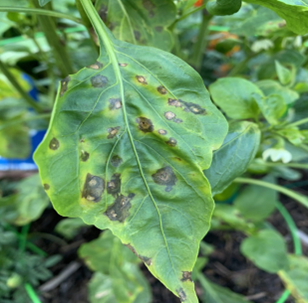
\includegraphics[width=\linewidth]{figures/Picture_test_Fast_SCNN.png}
    \caption{Fast-SCNN}
  \end{subfigure}
  \hfill
  \begin{subfigure}[b]{0.48\linewidth}
    \centering
    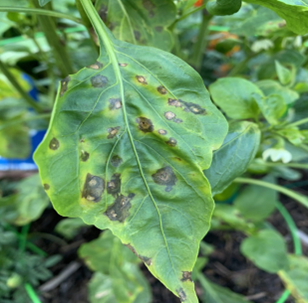
\includegraphics[width=\linewidth]{figures/Picture_test_enet.png}
    \caption{ENet}
  \end{subfigure}
  \caption{So sánh kết quả phân vùng trên tập kiểm tra (PC/GPU). Fast-SCNN cho kết quả phân vùng chính xác hơn ENet trên cùng mẫu ảnh đầu vào.}
  \label{fig:test_compare}
\end{figure}

\subsection{Kết quả hiệu năng trên Raspberry Pi 4}

Đây là phần đánh giá cốt lõi của nghiên cứu, phản ánh hiệu năng thực tế khi triển khai mô hình trên thiết bị biên đích. Quá trình đánh giá được thực hiện trên 50 ảnh kiểm tra, đo lường các chỉ số tốc độ, độ trễ và mức sử dụng tài nguyên.

\subsubsection{Tốc độ suy luận và Độ trễ}

Bảng~\ref{tab:pi_speed} so sánh hiệu năng suy luận của Fast-SCNN và ENet trên Raspberry Pi~4.

\begin{table}[htbp]
\centering
\caption{So sánh hiệu năng suy luận trên Raspberry Pi 4}
\label{tab:pi_speed}
\begin{tabular}{lccc}
\toprule
\textbf{Chỉ số} & \textbf{Fast-SCNN} & \textbf{ENet} & \textbf{Cải thiện} \\
\midrule
FPS trung bình        & \textbf{24,79} & 7,94   & 3,12$\times$ \\
Độ trễ TB (ms) & \textbf{40,33} & 125,94 & 3,12$\times$ \\
\bottomrule
\end{tabular}
\end{table}

Fast-SCNN đạt tốc độ suy luận \textbf{24,79~FPS} trên CPU ARM Cortex-A72, tương ứng với độ trễ trung bình \textbf{40,33~ms} cho mỗi khung hình. Đây là mức hiệu năng gần thời gian thực (near real-time), vượt ngưỡng 24~FPS --- tốc độ khung hình tối thiểu mà mắt người cảm nhận được chuyển động liên tục. Kết quả này đặc biệt ấn tượng khi xét rằng toàn bộ suy luận diễn ra trên CPU thuần, không có bất kỳ bộ tăng tốc phần cứng nào.

So với ENet, Fast-SCNN nhanh hơn \textbf{3,12 lần} (24,79~FPS so với 7,94~FPS). Kết quả này có vẻ trái ngược trực giác, bởi ENet có ít tham số hơn (0,36M so với 1,11M). Nguyên nhân được giải thích bởi hai yếu tố:

\begin{enumerate}
  \item \textbf{Tương thích toán tử với TFLite/XNNPACK.} Fast-SCNN sử dụng chủ yếu tích chập tách biệt theo chiều sâu --- loại toán tử được XNNPACK tối ưu hóa cao độ cho CPU ARM. Trong khi đó, ENet sử dụng một số toán tử phức tạp hơn (tích chập giãn bất đối xứng, tích chập chuyển vị) mà XNNPACK chưa tối ưu tốt, dẫn đến phải fallback về triển khai tham chiếu chậm hơn.
  \item \textbf{Kiến trúc thân thiện với bộ nhớ đệm.} Mô-đun Learning to Downsample của Fast-SCNN giảm kích thước không gian xuống 1/8 rất sớm trong pipeline, giúp các tầng phía sau xử lý bản đồ đặc trưng nhỏ, phù hợp với kích thước bộ nhớ đệm L1/L2 của ARM Cortex-A72.
\end{enumerate}

\subsubsection{Mức sử dụng tài nguyên}

Bảng~\ref{tab:ram} trình bày mức sử dụng RAM khi triển khai Fast-SCNN trên Raspberry Pi~4.

\begin{table}[htbp]
\centering
\caption{Mức sử dụng RAM trên Raspberry Pi 4}
\label{tab:ram}
\begin{tabular}{lc}
\toprule
\textbf{Chỉ số} & \textbf{Giá trị} \\
\midrule
RAM trước khi nạp mô hình   & 1.056,6 MB \\
RAM sau khi nạp và chạy      & 1.071,4 MB \\
RAM tăng thêm                & \textbf{14,8 MB} \\
Tỉ lệ sử dụng tổng cộng    & $\sim$26,8\% \\
\bottomrule
\end{tabular}
\end{table}

Mô hình Fast-SCNN sau lượng tử hóa chỉ tiêu thụ thêm \textbf{14,8~MB RAM} --- một mức cực kỳ thấp, chiếm chưa đến 0,4\% tổng bộ nhớ khả dụng 4~GB. Kết quả này cho thấy mô hình hoàn toàn an toàn về mặt bộ nhớ và để lại dư địa lớn cho hệ điều hành, các tiến trình nền, module tiền xử lý/hậu xử lý ảnh, và các ứng dụng đi kèm khác.

\subsubsection{Kết quả trực quan trên Raspberry Pi}

Hình~\ref{fig:inference_compare} minh họa kết quả suy luận thực tế của hai mô hình trên Raspberry Pi~4 với cùng ảnh đầu vào. Fast-SCNN phân vùng vùng bệnh chính xác hơn, với ranh giới rõ ràng và ít dương tính giả hơn so với ENet.

\begin{figure}[htbp]
  \centering
  \begin{subfigure}[b]{0.48\linewidth}
    \centering
    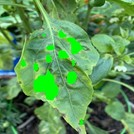
\includegraphics[width=\linewidth]{figures/Picture_inference_Fast_SCNN.jpg}
    \caption{Fast-SCNN trên Raspberry Pi}
  \end{subfigure}
  \hfill
  \begin{subfigure}[b]{0.48\linewidth}
    \centering
    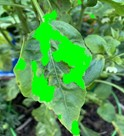
\includegraphics[width=\linewidth]{figures/Picture_inference_Enet.jpg}
    \caption{ENet trên Raspberry Pi}
  \end{subfigure}
  \caption{So sánh kết quả inference trên Raspberry Pi 4. Vùng xanh biểu thị mặt nạ phân vùng bệnh. Fast-SCNN cho kết quả phân vùng chính xác hơn với ranh giới rõ ràng, trong khi ENet có xu hướng phân vùng thừa (over-segmentation).}
  \label{fig:inference_compare}
\end{figure}

\subsection{Thảo luận chuyên sâu}

\subsubsection{Phân tích các trường hợp phân vùng tốt}

Mô hình Fast-SCNN cho thấy hiệu suất phân vùng xuất sắc trong các điều kiện sau:

\begin{itemize}
  \item \textbf{Độ tương phản cao giữa vùng bệnh và nền lá.} Khi các đốm bệnh có màu sắc đặc trưng, tương phản rõ ràng với bề mặt lá xanh, mô hình phân vùng chính xác với IoU cao. Ví dụ điển hình là trường hợp bệnh đốm vi khuẩn trên ớt chuông (Bell pepper bacterial spot), đạt \textbf{IoU~=~0,682} --- cao hơn mức trung bình 0,667. Các đốm bệnh màu nâu đen trên nền lá xanh tạo gradient cường độ mạnh, giúp các bộ lọc tích chập dễ dàng nhận diện ranh giới.
  \item \textbf{Điều kiện chụp lý tưởng.} Ảnh được chụp trong điều kiện ánh sáng đồng đều, nền ảnh đơn giản (chỉ có lá), và lá nằm trọn trong khung hình cho kết quả phân vùng tốt nhất.
\end{itemize}

\subsubsection{Phân tích các trường hợp hiệu suất giảm}

Mô hình gặp khó khăn và cho kết quả thấp hơn (IoU giảm xuống khoảng \textbf{0,659}) trong một số điều kiện cụ thể:

\begin{itemize}
  \item \textbf{Ánh sáng không đồng đều.} Khi ảnh chụp trong điều kiện ánh sáng tự nhiên ngoài trời, các vùng sáng tối không đều trên bề mặt lá có thể bị nhầm lẫn với các đốm bệnh, dẫn đến dương tính giả (false positives).
  \item \textbf{Bóng râm.} Bóng đổ từ các lá khác hoặc cành cây tạo ra các vùng tối cục bộ trên bề mặt lá. Mô hình đôi khi phân loại sai các vùng bóng râm thành vùng bệnh, đặc biệt khi bóng có hình dạng tương tự các đốm bệnh.
  \item \textbf{Che khuất bởi vật thể ngoài.} Khi lá bị tay người, dụng cụ nghiên cứu hoặc các lá khác che khuất một phần, mô hình gặp khó khăn trong việc xác định ranh giới chính xác giữa vùng bệnh, vùng bị che và nền.
\end{itemize}

\subsubsection{Phân tích tác động của lượng tử hóa}

Một kết quả đáng chú ý là mô hình sau lượng tử hóa INT8 vẫn duy trì hiệu suất phân vùng ở mức chấp nhận được (IoU~=~0,667), cho thấy quá trình ánh xạ từ FP32 sang INT8 không gây suy giảm nghiêm trọng chất lượng dự đoán. Điều này có thể được giải thích bởi:

\begin{enumerate}
  \item \textbf{Dư thừa thông tin trong trọng số.} Các trọng số của mô hình học sâu thường chứa mức độ dư thừa nhất định, cho phép nén mà không mất mát đáng kể thông tin hữu ích.
  \item \textbf{Đặc thù bài toán phân vùng nhị phân.} So với phân vùng đa lớp (multi-class), phân vùng nhị phân (bệnh/không bệnh) có yêu cầu phân biệt thấp hơn, giúp mô hình lượng tử hóa vẫn đủ năng lực biểu diễn cho ranh giới quyết định đơn giản hơn.
  \item \textbf{Kiến trúc tương thích lượng tử hóa.} Fast-SCNN chủ yếu sử dụng các toán tử được hỗ trợ tốt bởi TFLite, giảm thiểu lỗi lượng tử hóa tích lũy qua các tầng.
\end{enumerate}

\subsubsection{So sánh tổng hợp}

Bảng~\ref{tab:overall} tổng hợp toàn bộ kết quả so sánh giữa hai mô hình trên cả hai nền tảng.

\begin{table}[htbp]
\centering
\caption{So sánh tổng hợp Fast-SCNN và ENet}
\label{tab:overall}
\begin{tabular}{lccc}
\toprule
\textbf{Chỉ số} & \textbf{Fast-SCNN} & \textbf{ENet} & \textbf{Nhận xét} \\
\midrule
Số tham số              & 1,11M              & 0,36M & ENet nhẹ hơn 3$\times$ \\
IoU (PC)      & \textbf{0,667}     & 0,4195 & +59\% \\
FPS (RPi4)    & \textbf{24,79}     & 7,94 & +3,12$\times$ \\
Độ trễ (RPi4) & \textbf{40,33 ms}  & 125,94 ms & $-$3,12$\times$ \\
RAM tăng thêm           & \textbf{14,8 MB}   & -24 MB & Cực nhẹ \\
Dung lượng TFLite       & \textbf{636 KB}    & 204 KB & Sau INT8 PTQ \\
\bottomrule
\end{tabular}
\end{table}

Kết quả tổng hợp cho thấy Fast-SCNN vượt trội toàn diện so với ENet trên mọi chỉ số quan trọng: \textbf{chính xác hơn} (IoU cao hơn 59\%), \textbf{nhanh hơn} (FPS cao hơn 3,12 lần), và \textbf{nhẹ trên bộ nhớ} (chỉ tăng 14,8~MB RAM). Nghịch lý ``nhiều tham số hơn nhưng nhanh hơn'' được giải thích bởi sự tương thích kiến trúc với runtime XNNPACK và cấu trúc bộ nhớ đệm CPU ARM, như đã phân tích ở trên.

\subsubsection{Ý nghĩa thực tiễn}

Các kết quả thực nghiệm khẳng định rằng việc triển khai phân vùng bệnh thực vật gần thời gian thực trên Raspberry Pi~4 là \textbf{hoàn toàn khả thi} với chi phí phần cứng dưới 50~USD. Tốc độ 24,79~FPS đáp ứng yêu cầu xử lý video liên tục từ camera, cho phép xây dựng hệ thống giám sát bệnh tự động tại đồng ruộng mà không cần kết nối internet hay máy chủ đám mây. Mức tiêu thụ RAM cực thấp (14,8~MB) đảm bảo hệ thống hoạt động ổn định trong thời gian dài mà không gặp vấn đề tràn bộ nhớ --- yếu tố quan trọng đối với thiết bị IoT vận hành liên tục 24/7 trong điều kiện thực địa.


% ========== 5. KẾT LUẬN VÀ HƯỚNG PHÁT TRIỂN ==========
\section{Kết luận và Hướng phát triển}

\subsection{Kết luận}

Bài báo này trình bày một quy trình end-to-end hoàn chỉnh cho việc triển khai mô hình phân vùng ảnh ngữ nghĩa sử dụng học sâu trên thiết bị biên Raspberry Pi~4, hướng đến ứng dụng phát hiện bệnh thực vật trong nông nghiệp chính xác. Từ giai đoạn chuẩn bị dữ liệu, huấn luyện mô hình, lượng tử hóa đến triển khai và đánh giá trên thiết bị đích, toàn bộ quy trình đã được thiết kế, hiện thực hóa và kiểm chứng bằng số liệu thực nghiệm cụ thể.

Các kết quả chính đạt được bao gồm:
\begin{enumerate}
  \item \textbf{Triển khai thành công mô hình Fast-SCNN trên Raspberry Pi~4.} Mô hình được huấn luyện trên tập dữ liệu PlantSeg~v7 (7.774 ảnh) và chuyển đổi sang định dạng TensorFlow Lite thông qua lượng tử hóa INT8 sau huấn luyện, giảm dung lượng \textbf{75\%} (từ 2,5~MB xuống 636~KB).
  \item \textbf{Đạt hiệu năng suy luận gần thời gian thực.} Mô hình sau lượng tử hóa đạt tốc độ suy luận \textbf{24,79~FPS} với độ trễ trung bình \textbf{40,33~ms} trên CPU ARM Cortex-A72, vượt ngưỡng 24~FPS cho xử lý video liên tục. Mức tiêu thụ RAM chỉ tăng thêm \textbf{14,8~MB}, đảm bảo vận hành ổn định trên bộ nhớ 4~GB của thiết bị.
  \item \textbf{Duy trì độ chính xác phân vùng chấp nhận được.} Mô hình đạt chỉ số \textbf{IoU~=~0,667} trên tập kiểm tra 1.552 ảnh, chứng tỏ quá trình lượng tử hóa không gây suy giảm nghiêm trọng chất lượng dự đoán.
  \item \textbf{Vượt trội so với mô hình đối sánh.} Fast-SCNN cho kết quả cao hơn ENet trên mọi chỉ số: IoU cao hơn 59\% (0,667 so với 0,4195) và tốc độ suy luận nhanh hơn 3,12 lần (24,79~FPS so với 7,94~FPS) trên cùng thiết bị Raspberry Pi~4.
  \item \textbf{Đánh giá trên thiết bị đích thực tế.} Khác với phần lớn các nghiên cứu hiện hữu chỉ báo cáo chỉ số trên GPU máy chủ, toàn bộ quá trình đánh giá của chúng tôi được thực hiện trực tiếp trên CPU ARM --- cung cấp các số liệu FPS, độ trễ và RAM phản ánh chính xác hiệu năng triển khai trong điều kiện thực tế.
\end{enumerate}

Tổng hợp lại, nghiên cứu khẳng định rằng việc xây dựng hệ thống phân vùng bệnh thực vật gần thời gian thực trên phần cứng chi phí thấp (dưới 50~USD), không yêu cầu kết nối đám mây hay bộ tăng tốc AI chuyên dụng, là \textbf{hoàn toàn khả thi} --- mở ra tiềm năng ứng dụng Edge~AI trong giám sát nông nghiệp tại các vùng nông thôn và vùng sâu vùng xa.

\subsection{Hạn chế của nghiên cứu}

Mặc dù đạt được các kết quả tích cực, nghiên cứu vẫn tồn tại một số hạn chế cần được nhận thức rõ:

\begin{itemize}
  \item \textbf{Tiền xử lý cố định kích thước ảnh.} Toàn bộ ảnh đầu vào được resize về kích thước cố định $256 \times 256$ điểm ảnh trước khi đưa vào mô hình. Mặc dù kích thước này giúp giảm chi phí tính toán và đảm bảo tương thích với kiến trúc mạng, phép resize gây mất mát thông tin chi tiết đối với ảnh gốc có độ phân giải cao. Các đặc trưng bệnh nhỏ, các đốm bệnh ở giai đoạn sớm hoặc các kết cấu mịn trên bề mặt lá có thể bị mờ hoặc biến mất sau khi giảm kích thước, ảnh hưởng đến khả năng phân vùng chính xác ở mức chi tiết cao.
  \item \textbf{Chưa tận dụng bộ tăng tốc phần cứng.} Nghiên cứu hiện tại thực hiện toàn bộ suy luận trên CPU ARM mà chưa khai thác các bộ tăng tốc AI chuyên dụng như NPU hay Tensor Core. Mặc dù điều này phản ánh đúng thực trạng phần cứng của Raspberry Pi~4, việc bổ sung bộ tăng tốc ngoại vi có thể cải thiện đáng kể tốc độ suy luận.
  \item \textbf{Tập dữ liệu chưa mang tính địa phương hóa.} Tập dữ liệu PlantSeg~v7 chủ yếu bao gồm các loại bệnh trên cây trồng phổ biến quốc tế (ớt chuông, cà chua, khoai tây\ldots). Tập dữ liệu này \textbf{thiếu vắng các bệnh đặc trưng trên cây trồng chủ lực tại Việt Nam} như bệnh đạo ôn trên lúa, bệnh gỉ sắt trên cà phê, bệnh chảy mủ trên cao su, hay bệnh vàng lá greening trên cây có múi. Sự khác biệt về giống cây, điều kiện khí hậu nhiệt đới và chủng loại nấm/vi khuẩn gây bệnh đặc thù có thể ảnh hưởng đến khả năng tổng quát hóa của mô hình khi áp dụng tại Việt Nam.
\end{itemize}

\subsection{Hướng phát triển tương lai}

Dựa trên các kết quả đạt được và những hạn chế đã nhận diện, chúng tôi đề xuất các hướng phát triển sau:

\subsubsection{Nâng cấp nền tảng phần cứng}

\textbf{Chuyển đổi sang Raspberry Pi~5.} Thế hệ mới Raspberry Pi~5 được trang bị CPU ARM Cortex-A76 bốn nhân xung nhịp 2,4~GHz --- nhanh hơn khoảng 2--3 lần so với Cortex-A72 trên Pi~4. Việc triển khai mô hình trên Pi~5 dự kiến cải thiện đáng kể FPS, có khả năng đạt ngưỡng 50--60~FPS, đáp ứng yêu cầu thời gian thực nghiêm ngặt hơn.

\textbf{Tích hợp bộ tăng tốc Google Coral TPU.} Bộ đồng xử lý Coral Edge TPU (USB hoặc M.2) có khả năng thực hiện 4~TOPS (nghìn tỷ phép toán mỗi giây) cho các mô hình INT8, tiêu thụ chỉ 2W năng lượng. Việc kết hợp Coral TPU với Raspberry Pi sẽ giải phóng CPU cho các tác vụ khác và nâng tốc độ suy luận lên hàng trăm FPS.

\subsubsection{Xây dựng tập dữ liệu bệnh cây trồng Việt Nam}

Chúng tôi đề xuất thu thập một tập dữ liệu quy mô lớn gồm ít nhất 10.000 ảnh thực địa chụp tại các vùng trồng trọt trọng điểm tại Việt Nam, bao gồm: bệnh đạo ôn, bệnh bạc lá, bệnh khô vằn trên lúa (vùng Đồng bằng sông Cửu Long, Đồng bằng sông Hồng); bệnh gỉ sắt lá, bệnh nấm hồng trên cà phê (vùng Tây Nguyên); bệnh vàng lá greening, bệnh loét trên cây có múi (vùng Đồng bằng sông Cửu Long). Tập dữ liệu sẽ được chụp trong các điều kiện thực tế đa dạng nhằm nâng cao tính tổng quát và khả năng ứng dụng thực tiễn.

\subsubsection{Tích hợp hệ thống cảnh báo thời gian thực}

Để chuyển đổi từ nguyên mẫu nghiên cứu sang sản phẩm ứng dụng thực tế, chúng tôi đề xuất tích hợp giao thức truyền thông \textbf{MQTT (Message Queuing Telemetry Transport)} vào hệ thống. MQTT là giao thức nhắn tin nhẹ, phù hợp cho các thiết bị IoT với băng thông hạn chế. Quy trình hoạt động dự kiến: (1)~Raspberry Pi thực hiện phân vùng ảnh từ camera theo thời gian thực; (2)~Khi phát hiện vùng bệnh vượt ngưỡng diện tích cảnh báo, hệ thống tự động xuất bản thông báo lên MQTT broker; (3)~Ứng dụng di động trên điện thoại của nông dân nhận cảnh báo tức thì, bao gồm loại bệnh, mức độ nghiêm trọng, vị trí GPS và ảnh chụp minh chứng.

\subsubsection{Cải tiến kỹ thuật bổ sung}

Ngoài các hướng chính nêu trên, một số cải tiến kỹ thuật khác cũng đáng được khám phá:

\begin{itemize}
  \item \textbf{Phân vùng đa tỷ lệ (Multi-scale inference).} Áp dụng suy luận ở nhiều kích thước đầu vào và tổng hợp kết quả để cải thiện độ chính xác mà không cần thay đổi kiến trúc mô hình.
  \item \textbf{Tăng cường dữ liệu nâng cao.} Sử dụng các kỹ thuật tăng cường như CutMix, MixUp hoặc GAN-based augmentation để mở rộng tập huấn luyện, đặc biệt cho các lớp bệnh hiếm gặp.
  \item \textbf{Quantization-Aware Training (QAT).} Thay thế PTQ bằng QAT --- mô phỏng quá trình lượng tử hóa ngay trong lúc huấn luyện --- có khả năng khôi phục phần lớn độ chính xác bị mất do lượng tử hóa, đặc biệt khi chuyển sang các mô hình phức tạp hơn.
\end{itemize}

\subsection{Lời kết}

Nghiên cứu này đã chứng minh rằng ranh giới giữa trí tuệ nhân tạo hiệu năng cao và phần cứng chi phí thấp đang dần được thu hẹp. Với sự kết hợp giữa kiến trúc mô hình nhẹ, kỹ thuật lượng tử hóa và runtime tối ưu, việc đưa khả năng phân vùng ảnh học sâu --- vốn trước đây chỉ khả thi trên máy chủ GPU --- xuống một thiết bị nhỏ gọn, tiết kiệm năng lượng có giá dưới 50~USD không còn là viễn cảnh lý thuyết mà đã trở thành hiện thực có thể đo lường và tái tạo. Chúng tôi hy vọng rằng quy trình và kết quả được trình bày trong bài báo này sẽ đóng góp một phần vào việc đẩy nhanh quá trình ứng dụng Edge~AI trong nông nghiệp, đặc biệt tại các quốc gia đang phát triển như Việt Nam, nơi mà công nghệ chi phí thấp có thể mang lại tác động kinh tế-xã hội sâu rộng nhất.


% ========== TÀI LIỆU THAM KHẢO ==========
\bibliographystyle{IEEEtran}
\bibliography{references}

\end{document}